\subsection{Real-World Experimental Details} \label{sec:appendix_real}

Our real-world data used in experiments consists of 830 trajectories (61,482 transitions) collected by a human using a 3Dconnexion SpaceMouse device. Instructions for interfacing with the SpaceMouse is available publicly at \url{https://github.com/vitchyr/rlkit/tree/master/rlkit/demos/spacemouse}, with the device code adapted from the RoboSuite library~\cite{robosuite2020}. A full view of the robot and the view from the camera can be seen in Figure~\ref{fig:appendix_robot}.

Across our dataset, we interact with 10 drawer handles, 10 pot handles, 40 toys, and 60 distractor objects. Every 10 trajectories we randomly sample one or more interaction objects as well as two or more distractor objects. Before each rollout we randomize all object positions. The trajectories can be grouped into four separate categories: picking and placing toys, putting toys into a tray, opening a door and closing a drawer, and placing and removing a lid on a pot. To artificially increase the size of our dataset and make our policy robust to light changes and camera nudges, we utilize color jittering and random cropping during training. As there was an unequal amount of data per category, we re-balanced the dataset by using a different number of data augmentations per category. The final amount of task-specific data used per experiment is reported in Table~\ref{table:task-data-hyperparams}.

We additionally collected unscripted play data mixing all of the above behaviors with more object diversity, but did not use this data in this paper. With this data, there are 1,984 trajectories (137,111 transitions), covering 20 drawer handles, 20 pot handles, 60 toys, and 60 distractor objects. We also collected an additional 508 trajectories of on-policy robot data. The entire dataset is available on our website: \url{https://sites.google.com/view/val-rl}.

\begin{figure}[b]
%   \includegraphics[width=0.99\linewidth]{val/imgs/fig_pg1_v2.png}
  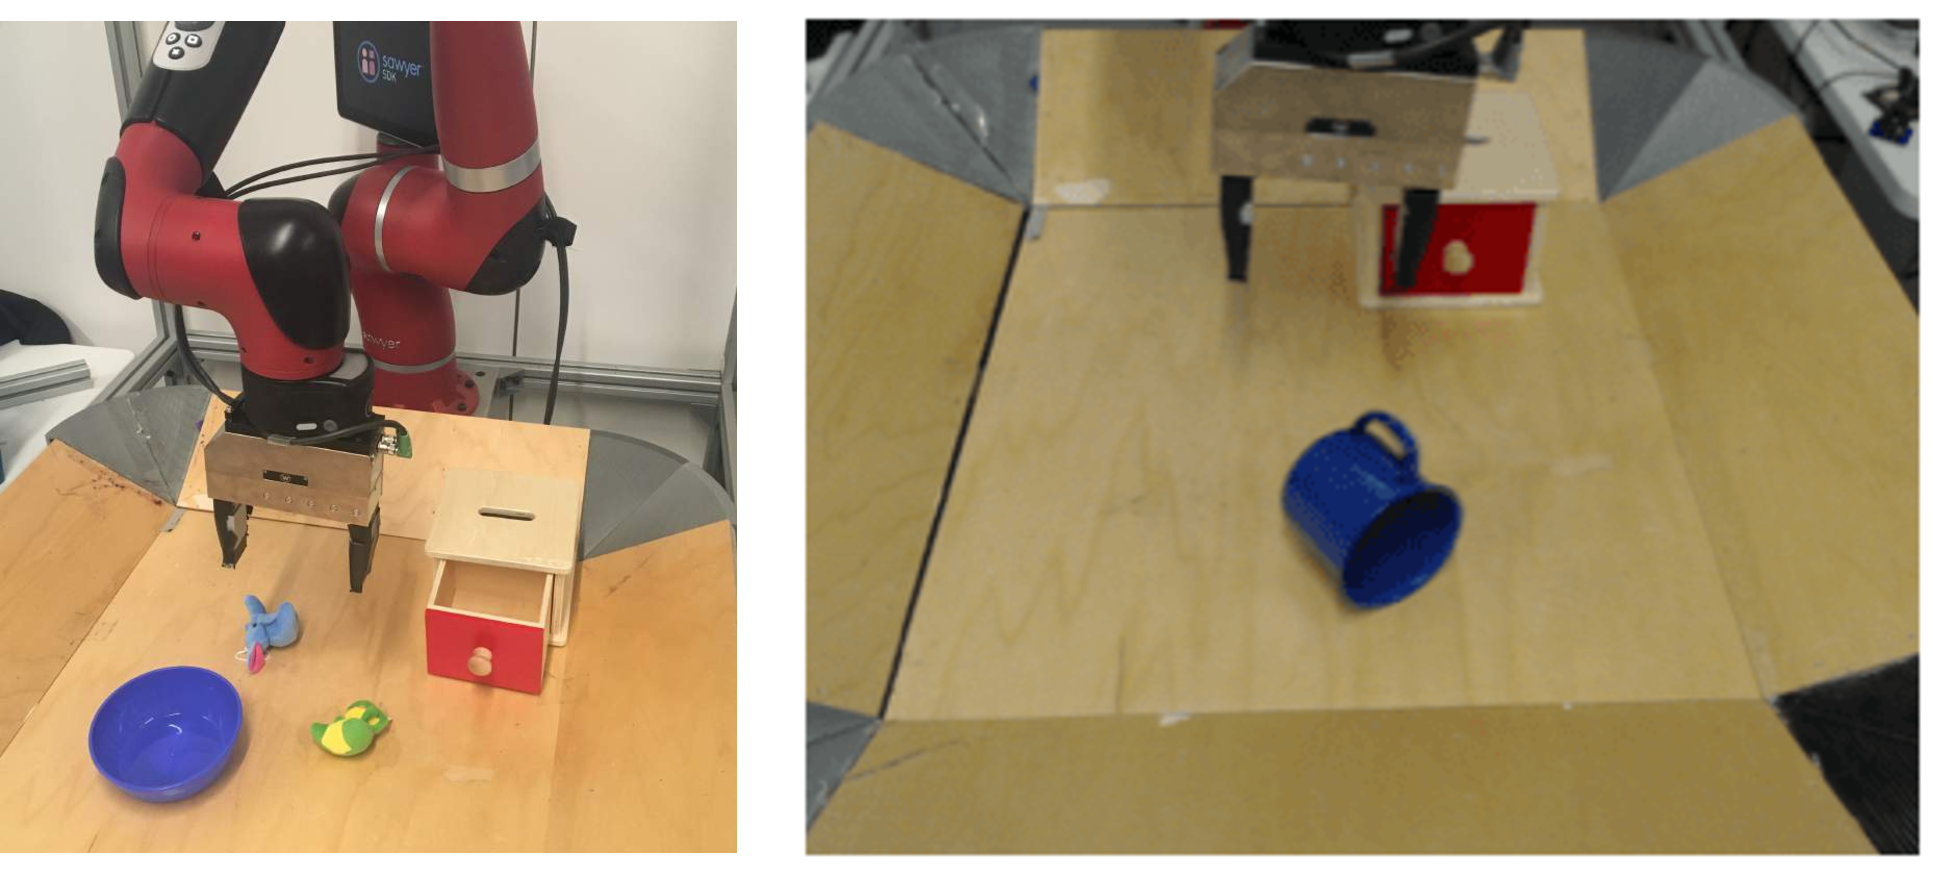
\includegraphics[width=0.99\linewidth]{val/imgs/fig_appendix_robot.pdf}
  \caption{\small
  Left, full view of Sawyer robot setup. Right, camera view.
  }
  \label{fig:appendix_robot}
  \vspace{-0.5cm}
\end{figure}

\begin{figure}
  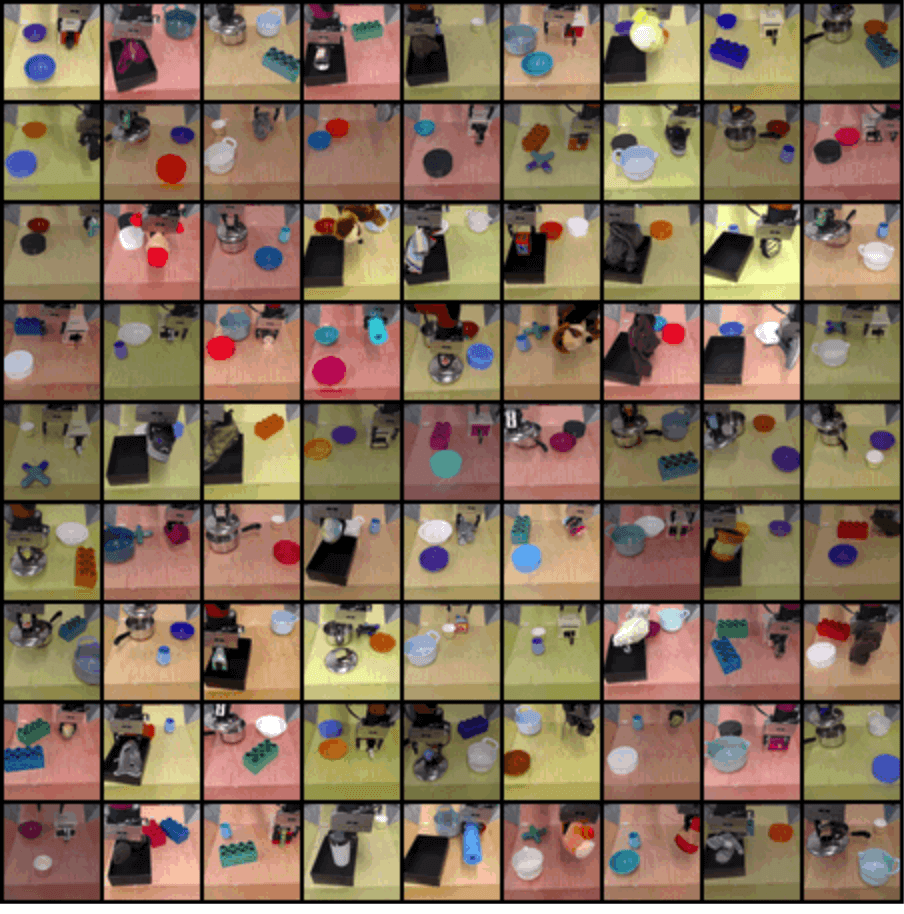
\includegraphics[width=0.99\linewidth]{val/imgs/prior_data_grid.png}
  \caption{\small
  Images from the prior dataset. The dataset contains 830 trajectories. We have released the full prior dataset (containing 1,984 trajectories) along with on-policy robot executions at our website, \url{https://sites.google.com/view/val-rl}
  }
  \label{fig:appendix_dataset_imgs}
  \vspace{-0.5cm}
\end{figure}

\subsection{Simulation Experimental Details} \label{sec:appendix_sim}

Our simulated dataset consists of 8,000 trajectories (400,000 transitions). Before sampling each trajectory, we randomize the existence, position, color, and orientation of the following: two drawers, a box, a button, and an object. If an object is present it is chosen from a set of 84 object geometries. The trajectories are generated by a scripted policy which collects play data by interacting with all the present objects in a random order. The scripted behavior includes: opening and closing a drawer by the handle, opening and closing a different drawer by pressing a button, and re-positioning objects. All simulated RL experiments were run with 5 seeds.

\subsection{Algorithm Details}

Visuomotor affordance learning (VAL) builds off the \texttt{rlkit} codebase available at \url{https://github.com/vitchyr/rlkit}. We will release our code at our website, \url{https://sites.google.com/view/val-rl}. Below, we list the specific hyperparameters used in our experiments for each component. In VAL, we first collect an offline data $\mathcal{D}$, run representation learning, then offline RL, and finally online RL for a specific environment.

In the representation learning phase, we first train the VQVAE~\cite{oord2017vqvae} on $\mathcal{D}$. We then encode the entire dataset with the VQVAE to obtain discrete latent variables, and then independently train the PixelCNN~\cite{oord2016pixelcnn} on discrete latent code dataset. For the CCRIG experiments, we train a CCVAE~\cite{sohn2015cvae} on $\mathcal{D}$.

In the offline RL phase, we run advantage weighted actor critic (AWAC)~\cite{nair2020awac} on the offline data to obtain a single policy and Q-function. This policy and Q-function can then be fine-tuned to a specific environment by running online RL. 

All hyperparameters are provided below for these algorithms are provided below in tables~\ref{table:awac-hyperparams}, \ref{table:data-hyperparams}, \ref{table:vqvae-hyperparams}, \ref{table:pixelcnn-hyperparams}, \ref{table:ccvae-hyperparams}.

\begin{table}[h!]
    \centering
    \begin{tabular}{c|c}
    \hline
    \textbf{Hyper-parameter} & \textbf{Value} \\
    \hline
    Training Batches Per Timestep & $1$\\
    Exploration Noise & None (stochastic policy) \\
    RL Batch Size & $1024$ \\
    Discount Factor & $0.99$\\
    Reward Scaling & $1$\\
    Replay Buffer Size & $1000000$\\
    Number of pretraining steps & $25000$ \\
    Policy Hidden Sizes & $[256, 256, 256, 256]$\\
    Policy Hidden Activation & ReLU\\
    Policy Weight Decay & $10^{-4}$ \\
    Policy Learning Rate & $3 \times 10^{-4}$\\
    Q Hidden Sizes & $[256, 256]$\\
    Q Hidden Activation & ReLU\\
    Q Weight Decay & $0$ \\
    Q Learning Rate & $3 \times 10^{-4}$\\
    Target Network $\tau$ & $5\times10^{-3}$ \\
    Relabeling strategy $p_\text{RS}(\zt)$ & 50\% future, 30\% prior, 20\% rollout \\
    \hline
    \end{tabular}
\caption{Hyper-parameters used for RL (AWAC) experiments.}
\label{table:awac-hyperparams}
\end{table}

\begin{table}[h!]
    \centering
    \begin{tabular}{c|c}
    \hline
    \textbf{Hyper-parameter} & \textbf{Value} \\
    \hline
    Brightness (Color Jitter) & $[0.75,1.25]$\\
    Contrast (Color Jitter) & $[0.9,1.1]$\\
    Saturation (Color Jitter) & $[0.9,1.1]$\\
    Hue (Color Jitter) & $[-0.1,0.1]$\\
    Size (Random Resized Crop) & $48$\\
    Scale (Random Resized Crop) & $[0.9, 1.0]$\\
    Ratio (Random Resized Crop) & $[0.9, 1.1]$\\
    Interpolation (Random Resized Crop) & Antialiasing\\
    \hline
    \end{tabular}
\caption{Hyper-parameters used for data augmentation.}
\label{table:data-hyperparams}
\end{table}

\begin{table}[h!]
    \centering
    \begin{tabular}{c|c}
    \hline
    \textbf{Hyper-parameter} & \textbf{Value} \\
    \hline
    Convolution Layers & $3$\\
    Convolution Hidden Size & $128$\\
    Residual Layers & $3$\\
    Residual Hidden Size & $64$\\
    Embedding Size & $5$\\
    Dictionary Size & $512$\\
    Commitment Cost & $0.25$\\
    EMA Embedding & $False$\\
    \hline
    \end{tabular}
\caption{Hyper-parameters used for VQVAE training.}
\label{table:vqvae-hyperparams}
\end{table}

\begin{table}[h!]
    \centering
    \begin{tabular}{c|c}
    \hline
    \textbf{Hyper-parameter} & \textbf{Value} \\
    \hline
    Batch Size & $32$\\
    Layers & $15$\\
    Learning Rate & $0.0003$\\
    Latent Conditioning Type & $Continuous$\\
    \hline
    \end{tabular}
\caption{Hyper-parameters used for PixelCNN experiments.}
\label{table:pixelcnn-hyperparams}
\end{table}

\begin{table}[h!]
    \centering
    \begin{tabular}{c|c}
    \hline
    \textbf{Hyper-parameter} & \textbf{Value} \\
    \hline
    Convolution Layers & $3$\\
    Convolution Hidden Size & $128$\\
    Residual Layers & $3$\\
    Residual Hidden Size & $64$\\
    Embedding Size & $5$\\
    Conditioning Embedding Size & $1$\\
    \hline
    \end{tabular}
\caption{Hyper-parameters used for CCVAE training.}
\label{table:ccvae-hyperparams}
\end{table}

\begin{table}[h!]
    \centering
    \begin{tabular}{c|c}
    \hline
    \textbf{Hyper-parameter} & \textbf{Value} \\
    \hline
    Tray & $25 \%$ task specific data\\
    Pick and Place & $25 \%$ task specific data\\
    Close Drawer & $20 \%$ task specific data\\
    Open Drawer & $20 \%$ task specific data\\
    Place Lid & $17 \%$ task specific data\\
    \hline
    \end{tabular}
\caption{Hyper-parameters used for task-specific replay buffer re-balancing (through data augmentation).}
\label{table:task-data-hyperparams}
\end{table}

\end{document}